\chapter{Практические задания}

\begin{enumerate}[wide=0pt]
\item \textit{Составить диаграмму вычисления следующих выражений::}
\begin{enumerate}[label=\arabic*)]
	\item \lstinline {(equal 3 (abs - 3))}
	\item \lstinline {(equal (+ 1 2) 3)}
	\item \lstinline {(equal (* 4 7) 21)}
	\item \lstinline {(equal (* 2 3) (+ 7 2))}
	\item \lstinline {(equal (- 7 3) (* 3 2))}
	\item \lstinline {(equal (abs (- 2 4)) 3)}
	
\end{enumerate}


\begin{figure}[ht!]
	\centering
	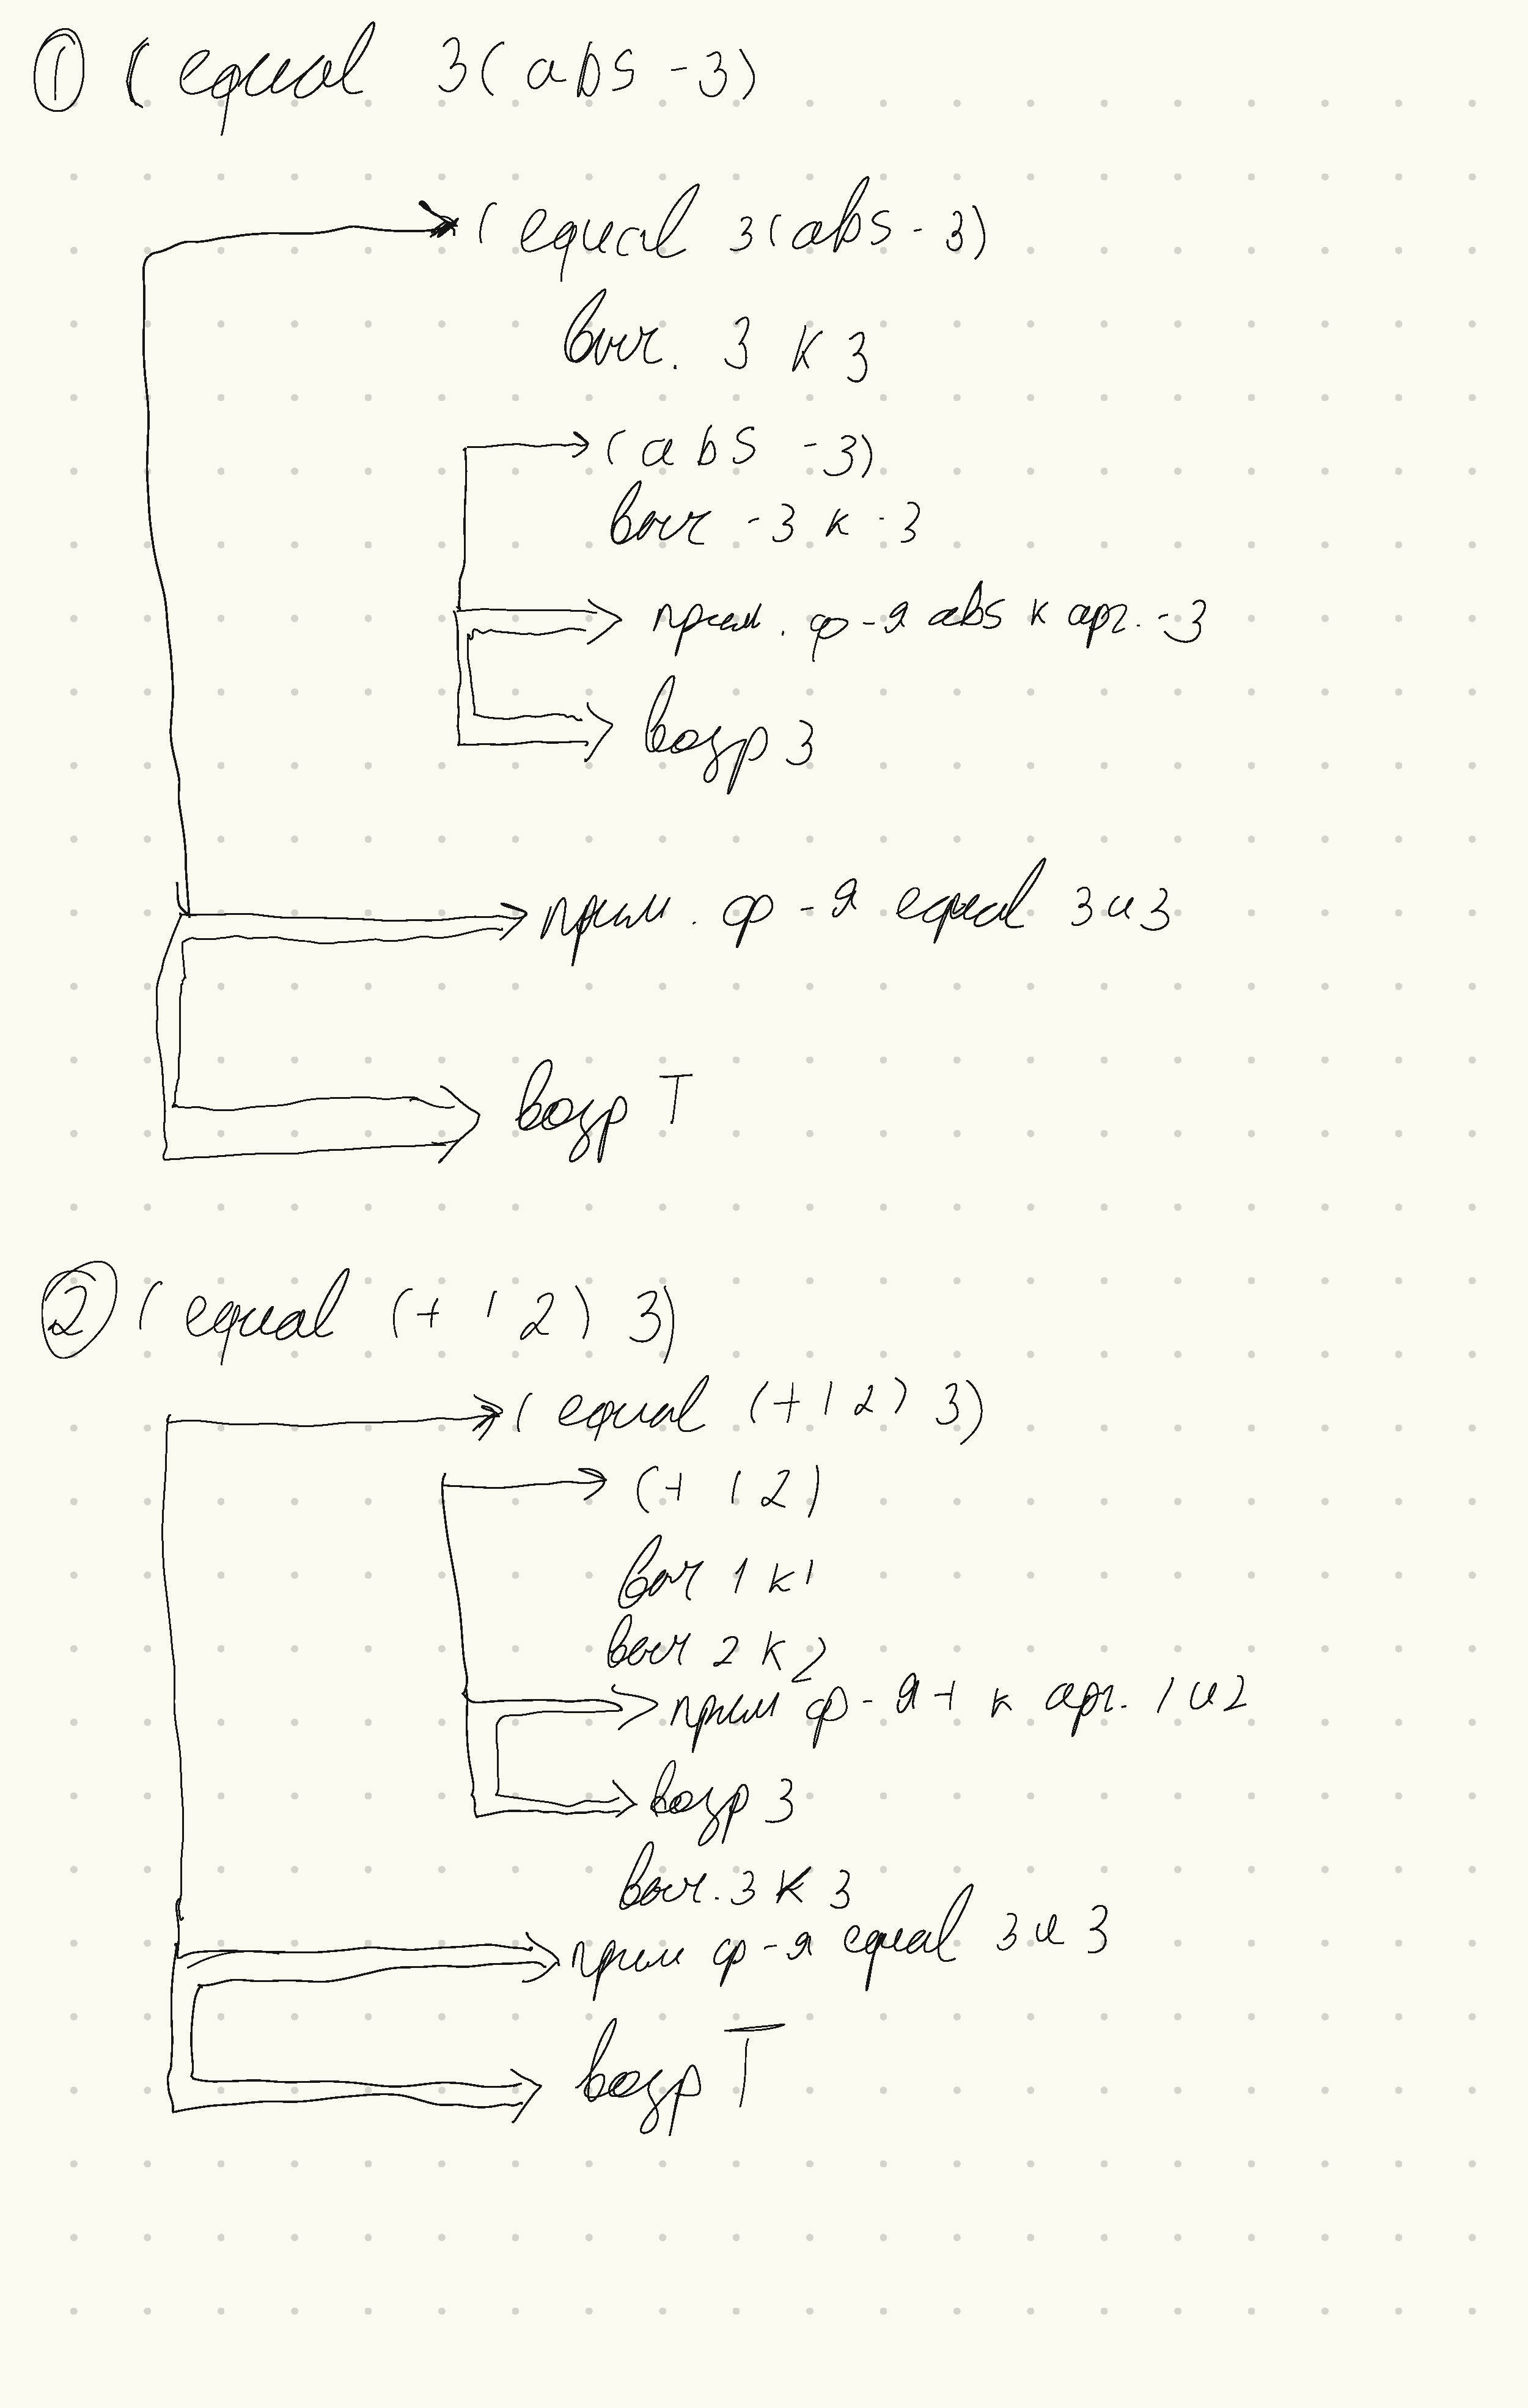
\includegraphics[width=1\linewidth]{assets/task1/1.pdf}
\end{figure}
\FloatBarrier

\begin{figure}[ht!]
	\centering
	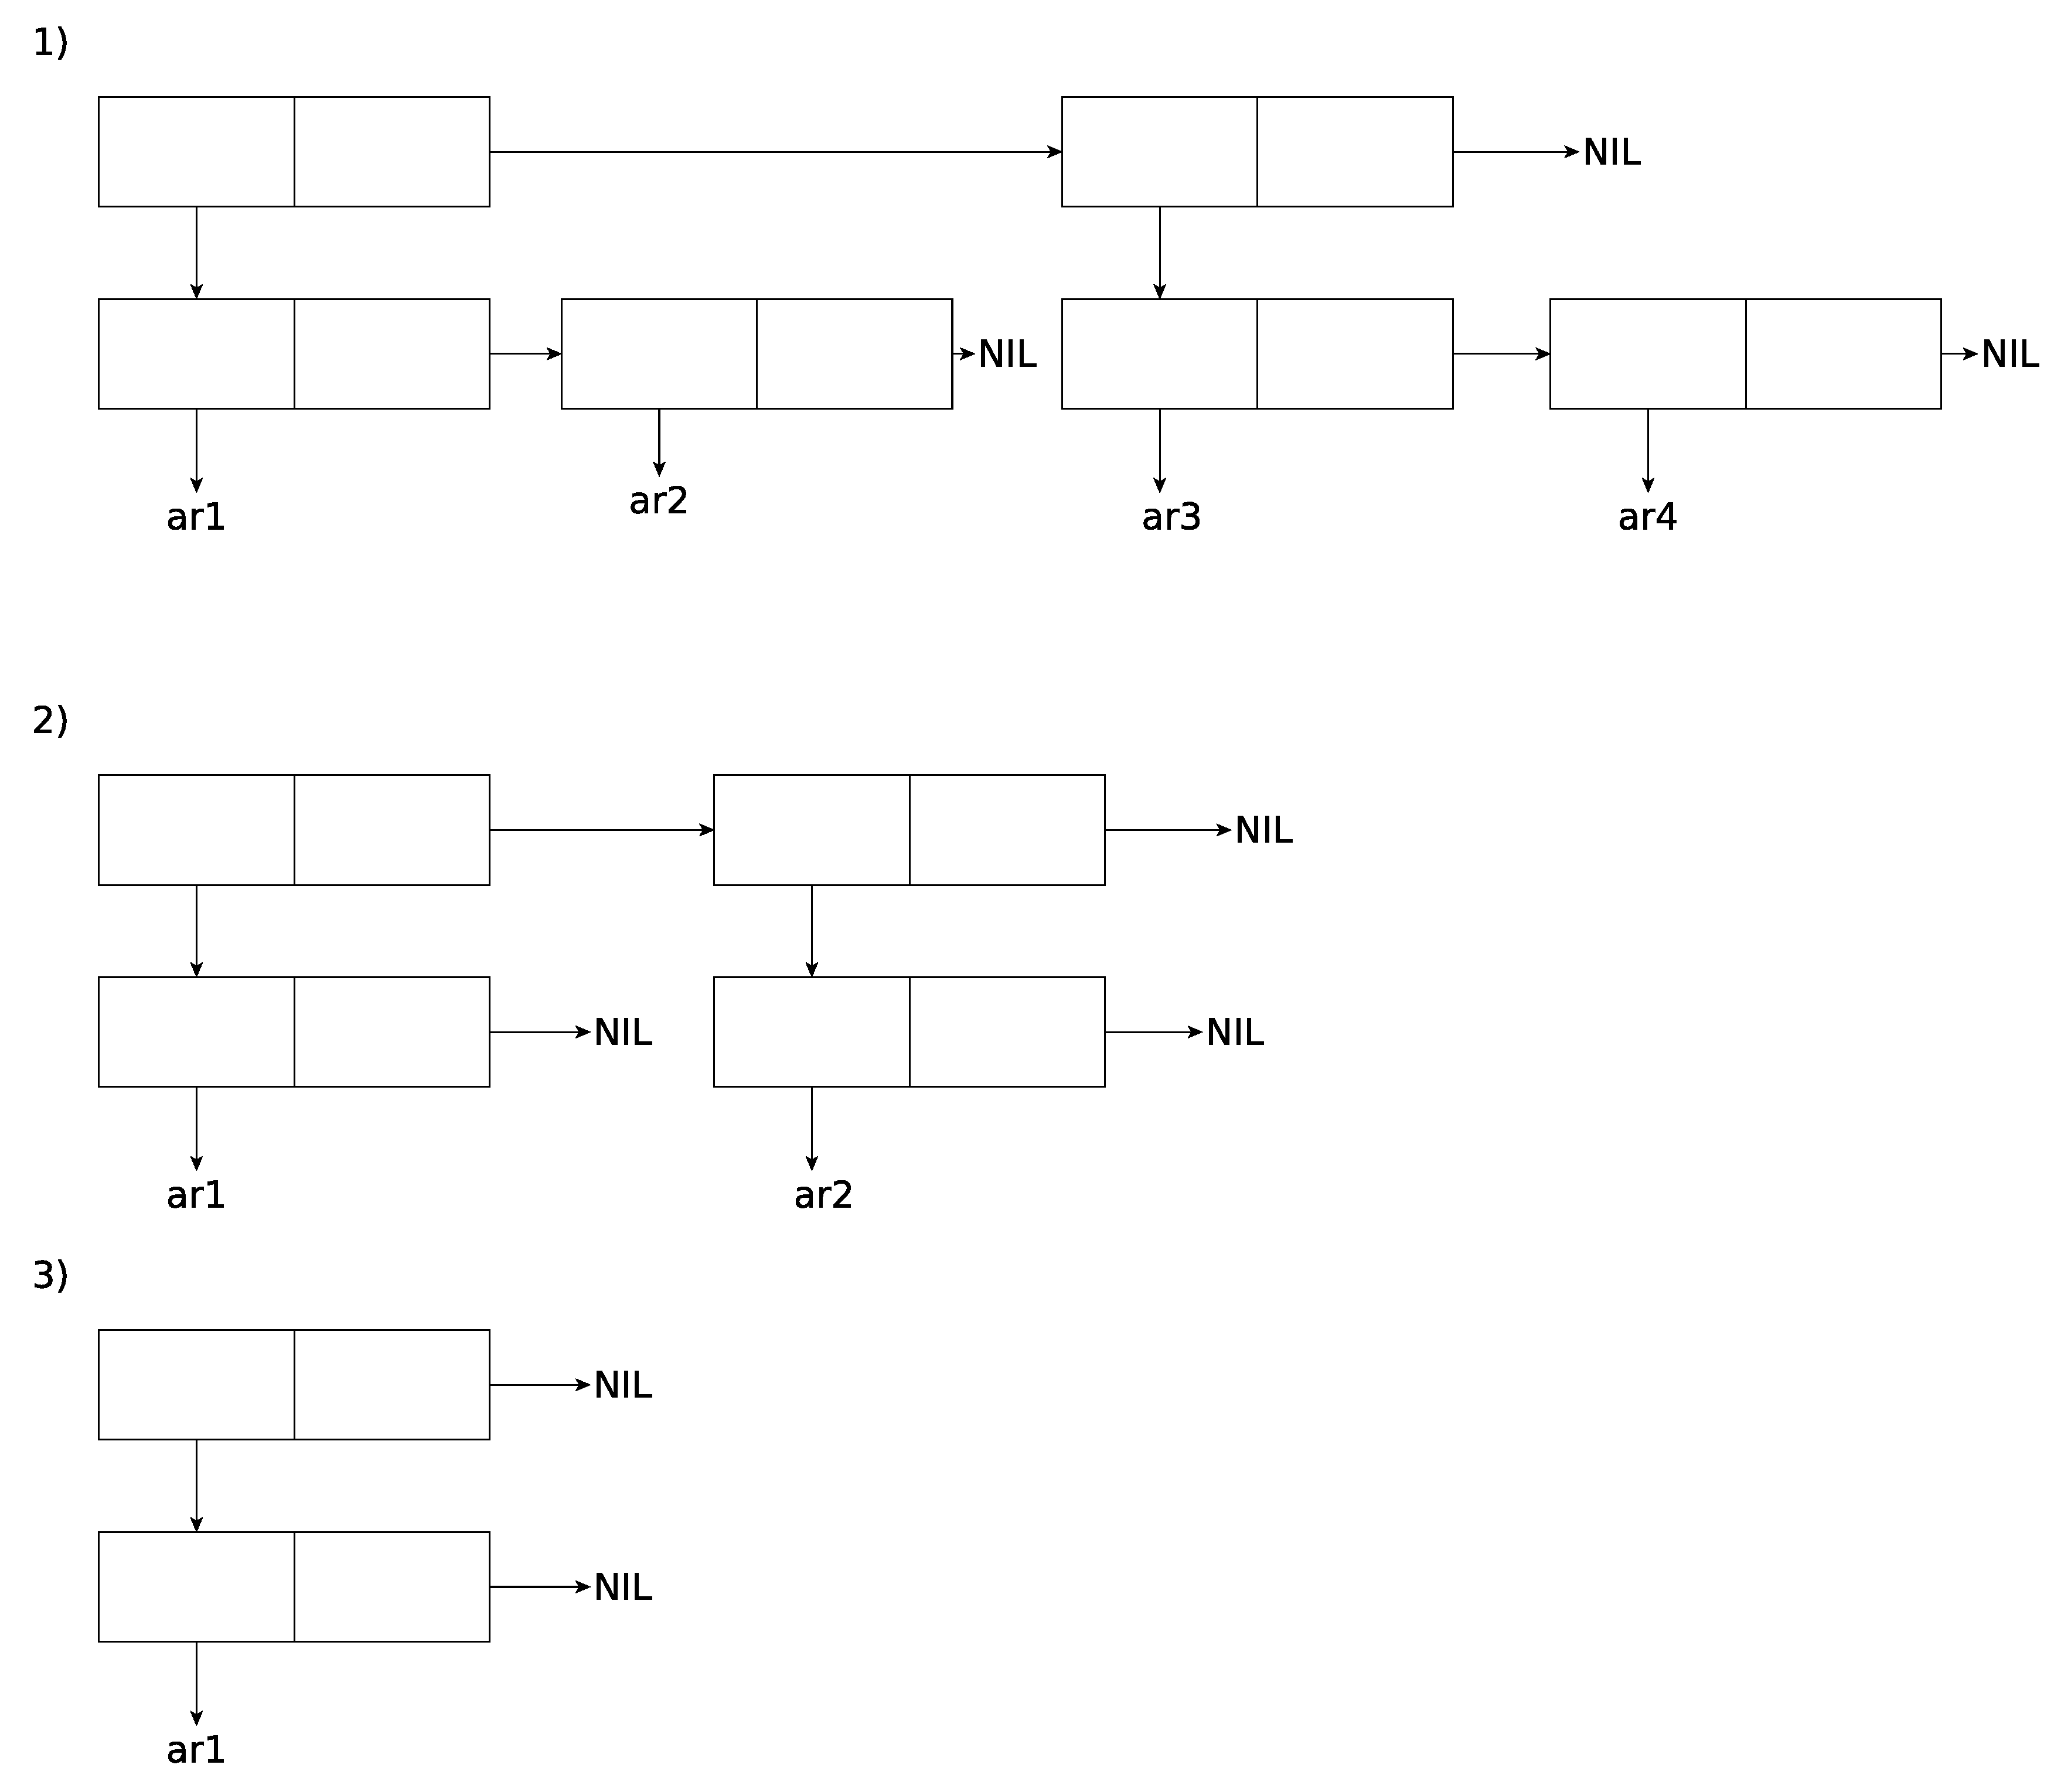
\includegraphics[width=1\linewidth]{assets/task1/2.pdf}
\end{figure}
\FloatBarrier
\begin{figure}[ht!]
	\centering
	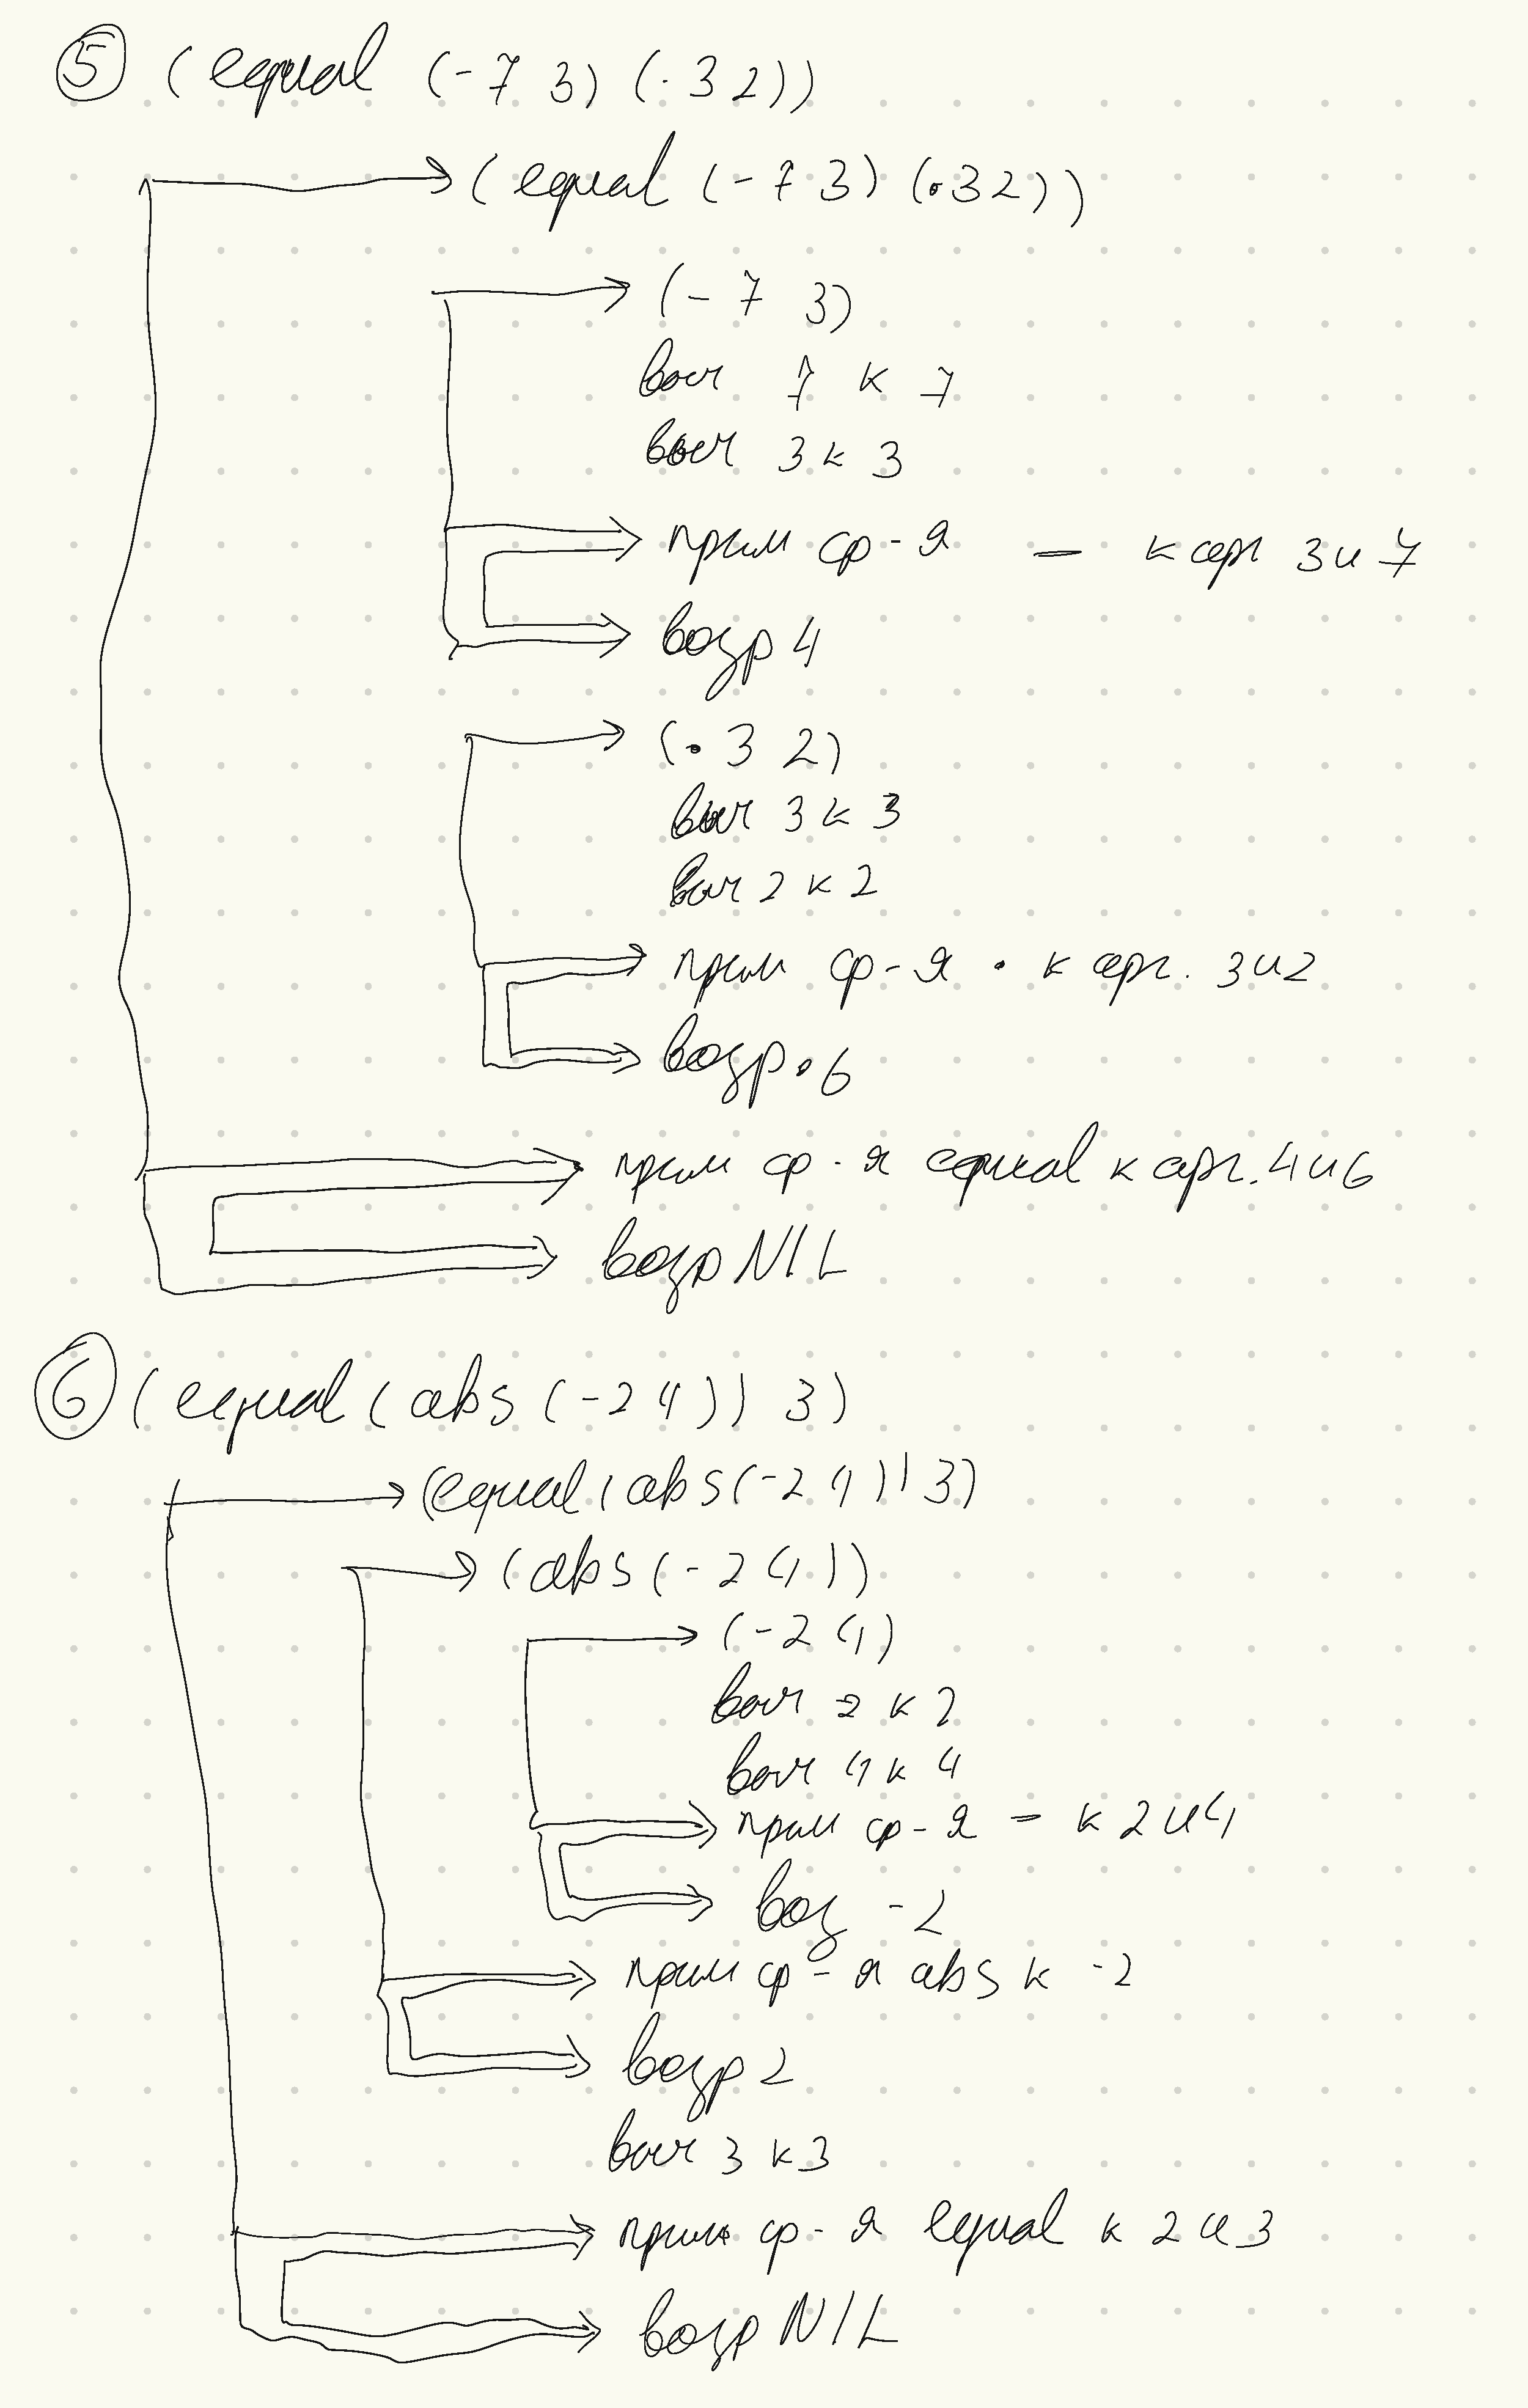
\includegraphics[width=1\linewidth]{assets/task1/3.pdf}
\end{figure}
\FloatBarrier



\item  \textit{Написать функцию, вычисляющую гипотенузу прямоугольного}

\begin{lstlisting}
	(
    defun calc_hyp(a b) (
        sqrt (
                + 
                    (* a a)
                    (* b b) 
            )
    )
	)

\end{lstlisting}


\item \textit{Каковы результаты вычисления следующих выражений?
(объяснить возможную ошибку и варианты ее устранен6ия)}

\begin{enumerate}[label=\arabic*)]
	\item \lstinline {(list 'a c)} --- 
	Результат: Ошибка. 
	Вариант решения: добавить ко второму аргументу quote.
	\item \lstinline {(cons 'a (b c))} --- 
	Результат: Ошибка. 
	Вариант решения: добавить ко второму аргументу quote.
	\item \lstinline {(cons 'a '(b c))} --- 
	Результат: (a b c) 
	\item \lstinline {(caddr (1 2 3 4 5))} --- 
	Результат: Ошибка. 
	Вариант решения: добавить quote.
	\item \lstinline {(cons 'a 'b 'c)} --- 
	Результат: Ошибка. 
	Вариант решения: убрать третий аргумент.
	\item \lstinline {(list 'a (b c))} --- 
	Результат: Ошибка. 
	Вариант решения: добавить quote к последниму аргументу.
	\item \lstinline {(list a '(b c))}  --- 
	Результат: Ошибка. 
	Вариант решения: добавить quote к первому аргументу.
	\item \lstinline {(list (+ 1 '(length '(1 2 3))))}  --- 
	Результат: Ошибка. 
	Вариант решения: убрать quote перед length. Тогда length будет интепритирована как функция, а не данные.
	
\end{enumerate}

\item \textit{Написать функцию longer\_then от двух списков-аргументов, 
которая возвращает T, если первый аргумент имеет большую длину.}


\begin{lstlisting}
	(defun longer_then(f s) (> (length f) (length s)))
\end{lstlisting}

\item \textit{Каковы результаты вычисления следующих выражений?}

\begin{enumerate}[label=\arabic*)]
	\item \lstinline {(cons 3 (list 5 6))} --- (3 5 6)
	\item \lstinline {(list 3 'from 9 'lives (- 9 3))} --- (3 from 9 lives 6)
	\item \lstinline {(+ (length for 2 too)) (car '(21 22 23)))} --- (Перменная for не определена)
	\item \lstinline {(cdr '(cons is short for ans))} --- (is short for ans)
	\item \lstinline {(car (list one two))} --- (Переменна one не определена)
	\item \lstinline {(cons 3 '(list 5 6))} --- (3 list for ans)
	\item \lstinline {(car (list 'one 'two))} --- one

	
\end{enumerate}

\item \textit{Дана функция (defun mystery (x) (list (second x) (first x))).
Какие результаты вычисления следующих выражений? }


\begin{enumerate}[label=\arabic*)]
	\item \lstinline {(mystery (one two))} --- one не определена.
	\item \lstinline {(mystery (last one two))} --- last не определена.
	\item \lstinline {(mystery free)} --- free не определена.
	\item \lstinline {(mystery one 'two))} --- one не определена.

	
\end{enumerate}

\item \textit{Написать функцию, которая переводит температуру в системе Фаренгейта
температуру по Цельсию (defum f-to-c (temp)…).
Формулы: 	c = 5/9*(f-320); 	f= 9/5*c+32.0. 
Как бы назывался роман Р.Брэдбери "+451 по Фаренгейту" в системе по Цельсию?}

\begin{lstlisting}
	(defun far-to-cel(temp) (* (/ 5 9)(- temp 32.0)))
\end{lstlisting}

Ответ: 232.77779 по Цельсию

\item \textit{Что получится при вычисления каждого из выражений?}


\begin{enumerate}[label=\arabic*)]
	\item \lstinline {(list 'cons t NIL)} --- (cons t NIL)
	\item \lstinline {(eval (eval (list 'cons t NIL)))} --- Переменная t не определена
	\item \lstinline {(apply #cons "(t NIL))} --- t
	\item \lstinline {(list 'eval NIL)} --- Неподдерживаемый синтаксис: \#cons
	\item \lstinline {(eval (list 'cons t NIL))} --- (eval NIL)
	\item \lstinline {(eval NIL)} --- NIL
	\item \lstinline {(eval (list 'eval NIL))} --- NIL

	
\end{enumerate}

\end{enumerate}